%Dạng 1
\setcounter{ex}{0}
\section{Tìm cực trị của hàm số dựa vào đồ thị}
\subsection{Kiến thức cần nhớ}
\begin{khung}
	\subsubsection{Định nghĩa}
Cho hàm số $y=f(x)$ xác định và liên tục trên khoảng $(a;b)$ (có thể $a$ là $-\infty$, $b$ là $+\infty$) và điểm $x_0\in (a;b)$.
\begin{itemize}
\item Nếu tồn tại số $h>0$ sao cho $f(x)<f(x_0)$ với mọi $x\in (x_0-h;x_0+h)$ và $x\neq x_0$ thì ta nói hàm số $f(x)$ đạt {\bf cực đại} tại $x_0$.
\item Nếu tồn tại số $h>0$ sao cho $f(x)>f(x_0)$ với mọi $x\in (x_0-h;x_0+h)$ và $x\neq x_0$ thì ta nói hàm số $f(x)$ đạt {\bf cực tiểu} tại $x_0$.
\end{itemize}
\begin{center}
\begin{tikzpicture}[scale=1, font=\footnotesize, line join=round, line cap=round,x=0.5cm,y=0.5cm,>=stealth]
\def \xmin{-4.5};
\def \xmax{6.5};
\def \ymin{-2.0};
\def \ymax{5.3};
\draw[->] (\xmin, 0.) -- (\xmax,0.) node[anchor=north] {$x$};
\draw[->] (0.,\ymin) -- (0.,\ymax) node[anchor=west] {$y$};
\clip(\xmin,\ymin) rectangle (\xmax,\ymax);
\begin{scope}
\draw[smooth,samples=100] plot[domain=\xmin+0.1:\xmax-0.1] (\x,{0.02*(\x)^5-0.1*(\x)^4-0.17*(\x)^3+0.9*(\x)^2+0.84*(\x)+1}) (5.5,4.7)node{$f(x)$};
\draw[dashed] (-2,0)node[below]{$x_\text{CĐ}$}|-(0,2)node[right]{$y_\text{CĐ}$} (4,0)node[below]{$x_\text{CT}$}|-(0,2.75)node[left]{$y_\text{CT}$};
\end{scope}
\draw[fill=black] (0,0) circle (1pt) node[below left] {$O$} (4,0) circle (1pt) (-2,0) circle (1pt) (0,2.75) circle (1pt) (-2,2) circle (1pt) (4,2.75) circle (1pt);
\end{tikzpicture}
\end{center}
\subsubsection{Chú ý}
\begin{enumerate}
\item  Nếu hàm số $f(x)$ đạt cực đại (cực tiểu) tại $x_0$ thì $x_0$ được gọi là điểm cực đại (điểm cực tiểu) của hàm số; $f\left(x_0\right)$ được gọi là giá trị cực đại (giá trị cực tiểu) của hàm số, kí hiệu là $y_\text{CĐ}$ ($y_\text{CT}$), còn điểm $M\left(x_0 ; f\left(x_0\right)\right)$ được gọi là điểm cực đại (điểm cực tiểu) của đồ thị.
\item Các điểm cực đại và cực tiểu được gọi chung là điểm cực trị. 
\end{enumerate}
\end{khung}
\subsection{Bài tập mẫu}
\Opensolutionfile{ans}[ans/ANS-DANG-27]
\setcounter{vd}{26}
\begin{khung}
	\begin{vd}[Đề tham khảo BGD 2022-2023]%[Cau27-GV14]%[2D1Y2-2]
\immini{Cho hàm số bậc ba $y=f(x)$ có đồ thị là đường cong trong hình bên. Giá trị cực đại của hàm số đã cho là
\choice
{$-1$}
{\True $3$}
{$2$}
{$0$}}{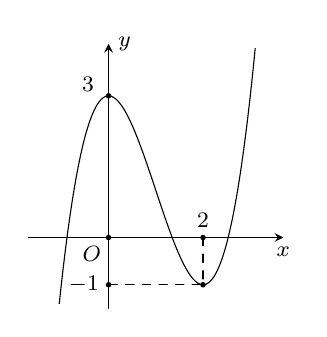
\begin{tikzpicture}[scale=1, font=\footnotesize, line join=round, line cap=round,>=stealth,x=0.6cm,y=0.6cm]
\def \xmin{-1.7};
\def \xmax{3.7};
\def \ymin{-1.5};
\def \ymax{4.1};
\draw[->] (\xmin, 0.) -- (\xmax,0.) node[anchor=north] {$x$};
\draw[->] (0.,\ymin) -- (0.,\ymax) node[anchor=west] {$y$};
\clip(\xmin+0.1,\ymin+0.1) rectangle (\xmax-0.1,\ymax-0.1);
\draw[smooth,samples=100,domain=\xmin:\xmax] plot(\x,{(\x-1)^3-3*(\x-1)+1});
\draw[dashed] (2,0) node[above]{$2$} |- (0,-1)node[left]{$-1$};
\foreach \x/\y in {2/0,0/-1,2/-1}{\fill[black] (\x,\y) circle(1pt);}
\foreach \x/\y/\l/\g  in {0/0/O/225,0/3/3/150}{\fill[black] (\x,\y) circle(1pt)+(\g:0.5) node{$\l$};}
\end{tikzpicture}}
\loigiai{
Từ đồ thị ta thấy hàm số $f(x)$ có giá trị cực đại là $y_\text{CĐ}=3$.
}
	\end{vd}
\end{khung}
\subsection{Bài tập tương tự và phát triển}

\begin{ex}%[Cau27-GV14]%[2D1Y2-2]
\immini{Cho hàm số $f(x)=ax^3+bx^2+cx+d$  có đồ thị như hình vẽ bên.
Mệnh đề nào sau đây {\bf sai}?
\choice
{Hàm số đạt cực đại tại $x=0$}
{Hàm số đạt cực tiểu tại $x=2$}
{\True Hàm số đạt cực đại tại $x=4$}
{Hàm số có hai điểm cực trị}}{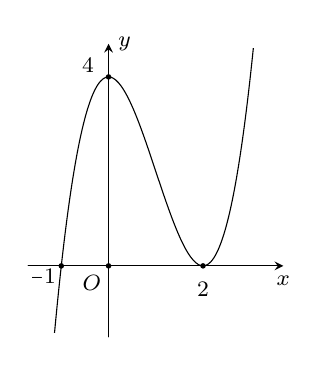
\begin{tikzpicture}[scale=1, font=\footnotesize, line join=round, line cap=round,>=stealth,x=0.6cm,y=0.6cm]
\def \xmin{-1.7};
\def \xmax{3.7};
\def \ymin{-1.5};
\def \ymax{4.7};
\draw[->] (\xmin, 0.) -- (\xmax,0.) node[anchor=north] {$x$};
\draw[->] (0.,\ymin) -- (0.,\ymax) node[anchor=west] {$y$};
\clip(\xmin+0.1,\ymin+0.1) rectangle (\xmax-0.1,\ymax-0.1);
\draw[smooth,samples=100,domain=\xmin:\xmax] plot(\x,{(\x-1)^3-3*(\x-1)+2});

\foreach \x/\y/\l/\g  in {0/0/O/225,2/0/2/-90,0/4/4/150,-1/0/-1/210}{\fill[black] (\x,\y) circle(1pt)+(\g:0.5) node{$\l$};}
\end{tikzpicture}}
\loigiai{
Từ đồ thị ta thấy hàm số $f(x)$ đạt cực đại tại $x=0$ nên mệnh đề  ``Hàm số đạt cực đại tại $x=4$'' là mệnh đề sai.
}
\end{ex}

\begin{ex}%[Cau27-GV14]%[2D1Y2-2]
\immini{Cho hàm số $y=f(x)$ liên tục trên $\mathbb{R}$ và có đồ thị như hình bên. Hỏi hàm số có bao nhiêu điểm cực trị?
\choice
{$2$}
{$3$}
{$4$}
{\True $5$}}{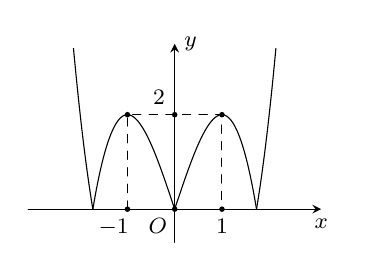
\begin{tikzpicture}[scale=1, font=\footnotesize, line join=round, line cap=round,>=stealth,x=0.6cm,y=0.6cm]
\def \xmin{-3.1};
\def \xmax{3.1};
\def \ymin{-0.7};
\def \ymax{3.5};
\draw[->] (\xmin, 0.) -- (\xmax,0.) node[anchor=north] {$x$};
\draw[->] (0.,\ymin) -- (0.,\ymax) node[anchor=west] {$y$};
\clip(\xmin+0.1,\ymin+0.1) rectangle (\xmax-0.1,\ymax-0.1);
\begin{scope}
\clip(\xmin+0.1,0) rectangle (0,\ymax-0.1);
\draw[smooth,samples=100,domain=\xmin:0] plot(\x,{(\x)^3-3*(\x)});
\end{scope}
\begin{scope}[xscale=-1]
\clip(\xmin+0.1,0) rectangle (0,\ymax-0.1);
\draw[smooth,samples=100,domain=\xmin:0] plot(\x,{(\x)^3-3*(\x)});
\end{scope}
\begin{scope}[yscale=-1]
\clip(\xmin+0.1,-3.5) rectangle (\xmax,0);
\draw[smooth,samples=100,domain=\xmin:0] plot(\x,{(\x)^3-3*(\x)});
\end{scope}
\begin{scope}[yscale=-1,xscale=-1]
\clip(\xmin+0.1,-3.5) rectangle (\xmax,0);
\draw[smooth,samples=100,domain=\xmin:0] plot(\x,{(\x)^3-3*(\x)});
\end{scope}
\draw[dashed] (-1,0) node[below,xshift=-5pt]{$-1$} |- (0,2)node[above left]{$2$}-|(1,0)node[below]{$1$};
\foreach \x/\y  in {-1/0,1/0,-1/2,1/2,0/2}{\fill[black] (\x,\y) circle(1pt);}
\foreach \x/\y/\l/\g  in {0/0/O/225}{\fill[black] (\x,\y) circle(1pt)+(\g:0.5) node{$\l$};}
\end{tikzpicture}}
\loigiai{
Dựa vào đồ thị hàm số ta thấy hàm số có $5$ điểm cực trị.
}
\end{ex}

\begin{ex}%[Cau27-GV14]%[2D1Y2-2]
\immini{Cho hàm số $y=ax^3+bx^2+cx+d$ có đồ thị như hình vẽ bên. Hàm số đã cho có bao nhiêu điểm cực trị?
\choice
{\True $2$}
{$1$}
{$3$}
{$4$}}{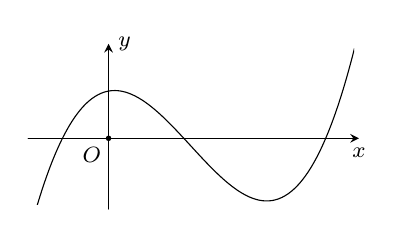
\begin{tikzpicture}[scale=1, font=\footnotesize, line join=round, line cap=round,>=stealth,x=0.6cm,y=0.6cm]
\def \xmin{-1.7};
\def \xmax{5.3};
\def \ymin{-1.5};
\def \ymax{2.0};
\draw[->] (\xmin, 0.) -- (\xmax,0.) node[anchor=north] {$x$};
\draw[->] (0.,\ymin) -- (0.,\ymax) node[anchor=west] {$y$};
\clip(\xmin+0.1,\ymin+0.1) rectangle (\xmax-0.1,\ymax-0.1);
\draw[smooth,samples=100,domain=\xmin:\xmax] plot(\x,{0.14*(\x)^3-0.73*(\x)^2+0.18*(\x)+1});
\foreach \x/\y/\l/\g  in {0/0/O/225}{\fill[black] (\x,\y) circle(1pt)+(\g:0.5) node{$\l$};}
\end{tikzpicture}}
\loigiai{
Từ đồ thị ta thấy hàm số đã cho có $2$ điểm cực trị.
}
\end{ex}

\begin{ex}%[Cau27-GV14]%[2D1Y2-2]
\immini{Cho hàm số $y=f(x)$ có đồ thị như hình vẽ bên. Tìm điểm cực đại của hàm số.
\choice
{$y=-2$}
{\True $x=-1$}
{$x=1$}
{$y=2$}}{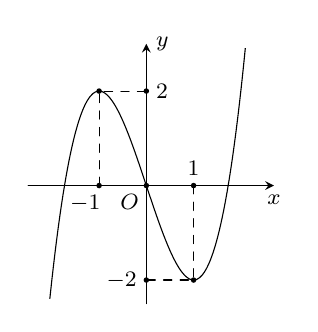
\begin{tikzpicture}[scale=1, font=\footnotesize, line join=round, line cap=round,>=stealth,x=0.6cm,y=0.6cm]
\def \xmin{-2.5};
\def \xmax{2.7};
\def \ymin{-2.5};
\def \ymax{3.0};
\draw[->] (\xmin, 0.) -- (\xmax,0.) node[anchor=north] {$x$};
\draw[->] (0.,\ymin) -- (0.,\ymax) node[anchor=west] {$y$};
\clip(\xmin+0.1,\ymin+0.1) rectangle (\xmax-0.1,\ymax-0.1);
\draw[smooth,samples=100,domain=\xmin:\xmax] plot(\x,{(\x)^3-3*(\x)});
\draw[dashed] (-1,0) node[below,xshift=-5pt]{$-1$} |- (0,2)node[right]{$2$} (1,0) node[above]{$1$} |- (0,-2)node[left]{$-2$};
\foreach \x/\y  in {-1/0,1/0,-1/2,1/-2,0/2,0/-2}{\fill[black] (\x,\y) circle(1pt);}
\foreach \x/\y/\l/\g  in {0/0/O/225}{\fill[black] (\x,\y) circle(1pt)+(\g:0.5) node{$\l$};}
\end{tikzpicture}}

\loigiai
{Từ đồ thị ta thấy hàm số đạt cực đại tại điểm $x=-1$.
}
\end{ex}

\begin{ex}%[Cau27-GV14]%[2D1B2-2]
\immini{Cho hàm số $y=f(x)$. Đồ thị hàm số $y=f'(x)$ như hình bên. Tìm mệnh đề đúng.
\choice
{Hàm số $y=f(x)$ nghịch biến trên khoảng $(0;2)$}
{Hàm số $y=f(x)$ có hai cực trị}
{Hàm số $y=f(x)$ đạt cực tiểu tại $x=2$}
{\True Hàm số $y=f(x)$ chỉ có một cực trị}}{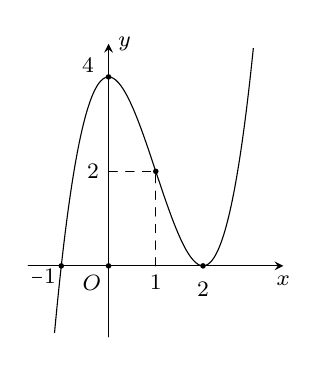
\begin{tikzpicture}[scale=1, font=\footnotesize, line join=round, line cap=round,>=stealth,x=0.6cm,y=0.6cm]
\def \xmin{-1.7};
\def \xmax{3.7};
\def \ymin{-1.5};
\def \ymax{4.7};
\draw[->] (\xmin, 0.) -- (\xmax,0.) node[anchor=north] {$x$};
\draw[->] (0.,\ymin) -- (0.,\ymax) node[anchor=west] {$y$};
\clip(\xmin+0.1,\ymin+0.1) rectangle (\xmax-0.1,\ymax-0.1);
\draw[smooth,samples=100,domain=\xmin:\xmax] plot(\x,{(\x-1)^3-3*(\x-1)+2});
\draw[dashed] (1,0) node[below]{$1$} |- (0,2)node[left]{$2$};
\fill[black] (1,2) circle(1pt);
\foreach \x/\y/\l/\g  in {0/0/O/225,2/0/2/-90,0/4/4/150,-1/0/-1/210}{\fill[black] (\x,\y) circle(1pt)+(\g:0.5) node{$\l$};}
\end{tikzpicture}}
\loigiai{
Từ đồ thị của hàm số $y=f'(x)$ ta có bảng xét dấu của $f'(x)$ như sau
\begin{center}

\begin{tikzpicture}
\tkzTabInit[nocadre=false, lgt=1.2, espcl=2.5, deltacl=0.6]{$x$/0.6,$f'(x)$/0.6}
{$-\infty$, $-1$, $2$, $+\infty$}
\tkzTabLine {,-,0,+,0,+,}
\end{tikzpicture}
\end{center}
Do đó hàm số $y=f(x)$ chỉ có một cực trị.
}
\end{ex}

\begin{ex}%[Cau27-GV14]%[2D1Y2-2]
\immini{Cho hàm số $f(x)$ xác định, liên tục trên tập số thực $\mathbb{R}$ và có đồ thị như hình bên. Hàm số $y=f(x)$
đạt cực tiểu tại điểm nào dưới đây?
\choice
{$x=0$}
{$x=-2$ và $x=0$}
{\True $x=-2$}
{$x=1$}}{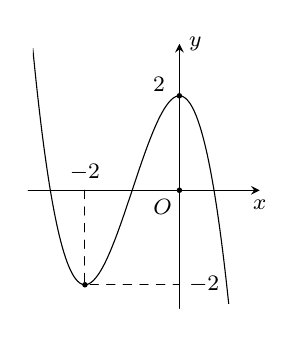
\begin{tikzpicture}[scale=1, font=\footnotesize, line join=round, line cap=round,>=stealth,x=0.6cm,y=0.6cm]
\def \xmin{-3.2};
\def \xmax{1.7};
\def \ymin{-2.5};
\def \ymax{3.1};
\draw[->] (\xmin, 0.) -- (\xmax,0.) node[anchor=north] {$x$};
\draw[->] (0.,\ymin) -- (0.,\ymax) node[anchor=west] {$y$};
\clip(\xmin+0.1,\ymin+0.1) rectangle (\xmax-0.1,\ymax-0.1);
\draw[smooth,samples=100,domain=\xmin:\xmax] plot(\x,{-(\x+1)^3+3*(\x+1)});
\draw[dashed] (-2,0) node[above]{$-2$} |- (0,-2)node[right]{$-2$};
\fill[black] (-2,-2) circle(1pt);
\foreach \x/\y/\l/\g  in {0/0/O/225,0/2/2/150}{\fill[black] (\x,\y) circle(1pt)+(\g:0.5) node{$\l$};}
\end{tikzpicture}}
\loigiai{
Dựa vào đồ thị hàm số $y=f(x)$, ta thấy hàm số đạt cực tiểu tại $x=-2$.
}
\end{ex}

\begin{ex}%[Cau27-GV14]%[2D1Y2-2]
\immini{Tìm điểm cực tiểu của hàm số $y=f(x)$, biết hàm số $y=f(x)$ có đồ thị như hình vẽ.
\choice
{$x=0$}
{$x=-2$}
{$x=1$}
{\True $x=2$}}{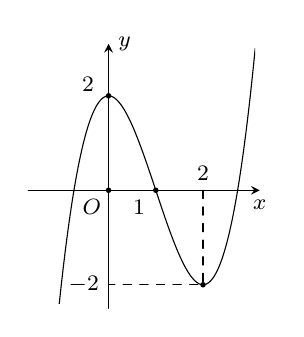
\begin{tikzpicture}[scale=1, font=\footnotesize, line join=round, line cap=round,>=stealth,x=0.6cm,y=0.6cm]
\def \xmin{-1.7};
\def \xmax{3.2};
\def \ymin{-2.5};
\def \ymax{3.1};
\draw[->] (\xmin, 0.) -- (\xmax,0.) node[anchor=north] {$x$};
\draw[->] (0.,\ymin) -- (0.,\ymax) node[anchor=west] {$y$};
\clip(\xmin+0.1,\ymin+0.1) rectangle (\xmax-0.1,\ymax-0.1);
\draw[smooth,samples=100,domain=\xmin:\xmax] plot(\x,{(\x-1)^3-3*(\x-1)});
\draw[dashed] (2,0) node[above]{$2$} |- (0,-2)node[left]{$-2$};
\fill[black] (2,-2) circle(1pt);
\foreach \x/\y/\l/\g  in {0/0/O/225,0/2/2/150,1/0/1/225}{\fill[black] (\x,\y) circle(1pt)+(\g:0.5) node{$\l$};}
\end{tikzpicture}}
\loigiai{Dựa vào đồ thị, ta thấy hàm số đạt cực tiểu tại $x=2$.}
\end{ex}

\begin{ex}%[Cau27-GV14]%[2D1Y2-2]
\immini{Cho hàm đa thức bậc ba $y=f(x)$ có đồ thị như hình vẽ bên. Biết hàm số $f(x)$ có các điểm cực trị là $x_1$, $x_2$. Tích $x_1x_2$ bằng
\choice
{$4$}
{\True $0$}
{$-4$}
{$-2$}}{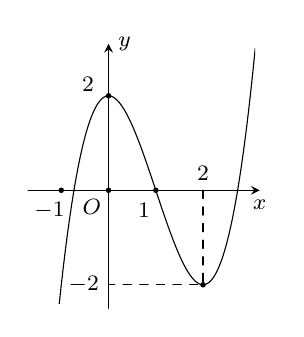
\begin{tikzpicture}[scale=1, font=\footnotesize, line join=round, line cap=round,>=stealth,x=0.6cm,y=0.6cm]
\def \xmin{-1.7};
\def \xmax{3.2};
\def \ymin{-2.5};
\def \ymax{3.1};
\draw[->] (\xmin, 0.) -- (\xmax,0.) node[anchor=north] {$x$};
\draw[->] (0.,\ymin) -- (0.,\ymax) node[anchor=west] {$y$};
\clip(\xmin+0.1,\ymin+0.1) rectangle (\xmax-0.1,\ymax-0.1);
\draw[smooth,samples=100,domain=\xmin:\xmax] plot(\x,{(\x-1)^3-3*(\x-1)});
\draw[dashed] (2,0) node[above]{$2$} |- (0,-2)node[left]{$-2$};
\fill[black] (2,-2) circle(1pt);
\foreach \x/\y/\l/\g  in {0/0/O/225,0/2/2/150,1/0/1/-120,-1/0/-1/-120}{\fill[black] (\x,\y) circle(1pt)+(\g:0.5) node{$\l$};}
\end{tikzpicture}}
 \loigiai{
Dựa vào đồ thị, ta thấy hàm số $f(x)$ có điểm cực đại $x=0$ và điểm cực tiểu $x=2$.\\
Vậy tích các điểm cực đại và cực tiểu của hàm số $f(x)$ là $0\times 2=0$.
}
\end{ex}

\begin{ex}%[Cau27-GV14]%[2D1Y2-2]
\immini{Cho đồ thị hàm số như hình vẽ bên. Giá trị cực đại của hàm số là
\choice
{\True $1$}
{$4$}
{$-1$}
{$-3$}}{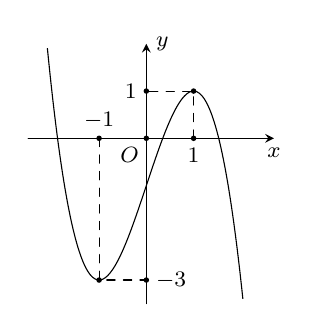
\begin{tikzpicture}[scale=1, font=\footnotesize, line join=round, line cap=round,>=stealth,x=0.6cm,y=0.6cm]
\def \xmin{-2.5};
\def \xmax{2.7};
\def \ymin{-3.5};
\def \ymax{2.0};
\draw[->] (\xmin, 0.) -- (\xmax,0.) node[anchor=north] {$x$};
\draw[->] (0.,\ymin) -- (0.,\ymax) node[anchor=west] {$y$};
\clip(\xmin+0.1,\ymin+0.1) rectangle (\xmax-0.1,\ymax-0.1);
\draw[smooth,samples=100,domain=\xmin:\xmax] plot(\x,{-(\x)^3+3*(\x)-1});
\draw[dashed] (-1,0) node[above]{$-1$} |- (0,-3)node[right]{$-3$} (1,0) node[below]{$1$} |- (0,1)node[left]{$1$};
\foreach \x/\y  in {-1/-3, 1/1,-1/0,1/0,0/1,0/-3}{\fill[black] (\x,\y) circle(1pt);}
\foreach \x/\y/\l/\g  in {0/0/O/225}{\fill[black] (\x,\y) circle(1pt)+(\g:0.5) node{$\l$};}
\end{tikzpicture}}
\loigiai{
Dựa vào đồ thị ta thấy được điểm cực đại của đồ thị có tọa độ là $(1;1)$ nên giá trị cực đại của hàm số là $y_\text{CĐ}=1$.}
\end{ex}

\begin{ex}%[Cau27-GV14]%[2D1Y2-2]
\immini{Cho hàm số $y=f(x)$ có đồ thị như hình vẽ bên. Mệnh đề nào dưới đây đúng?
\choice
{Giá trị cực đại của hàm số là $0$}
{\True Giá trị cực tiểu của hàm số bằng $-1$}
{Điểm cực tiểu của hàm số là $-1$}
{Điểm cực đại của hàm số là $3$}}{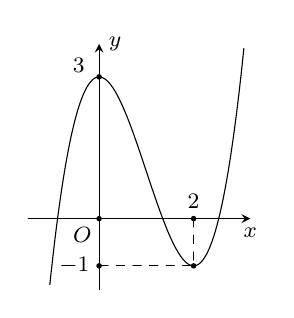
\begin{tikzpicture}[scale=1, font=\footnotesize, line join=round, line cap=round,>=stealth,x=0.6cm,y=0.6cm]
\def \xmin{-1.5};
\def \xmax{3.2};
\def \ymin{-1.5};
\def \ymax{3.7};
\draw[->] (\xmin, 0.) -- (\xmax,0.) node[anchor=north] {$x$};
\draw[->] (0.,\ymin) -- (0.,\ymax) node[anchor=west] {$y$};
\clip(\xmin+0.1,\ymin+0.1) rectangle (\xmax-0.1,\ymax-0.1);
\draw[smooth,samples=100,domain=\xmin:\xmax] plot(\x,{(\x-1)^3-3*(\x-1)+1});
\draw[dashed] (2,0) node[above]{$2$} |- (0,-1)node[left]{$-1$};
\foreach \x/\y  in {2/-1,2/0,0/-1}{\fill[black] (\x,\y) circle(1pt);}
\foreach \x/\y/\l/\g  in {0/0/O/225,0/3/3/150}{\fill[black] (\x,\y) circle(1pt)+(\g:0.5) node{$\l$};}
\end{tikzpicture}}
\loigiai{
Từ đồ thị ta thấy giá trị cực tiểu của hàm số bằng $-1$.
}
\end{ex}

\begin{ex}%[Cau27-GV14]%[2D1Y2-2]
\immini{Cho hàm số $y=ax^4+bx^2+c$, $(a\neq 0)$ có đồ thị như hình vẽ bên. Số điểm cực đại của hàm số là
\choice
{$3$}
{$4$}
{$1$}
{\True $2$}}{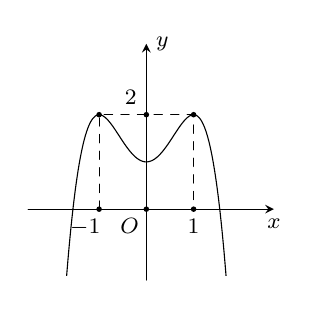
\begin{tikzpicture}[scale=1, font=\footnotesize, line join=round, line cap=round,>=stealth,x=0.6cm,y=0.6cm]
\def \xmin{-2.5};
\def \xmax{2.7};
\def \ymin{-1.5};
\def \ymax{3.5};
\draw[->] (\xmin, 0.) -- (\xmax,0.) node[anchor=north] {$x$};
\draw[->] (0.,\ymin) -- (0.,\ymax) node[anchor=west] {$y$};
\clip(\xmin+0.1,\ymin+0.1) rectangle (\xmax-0.1,\ymax-0.1);
\draw[smooth,samples=100,domain=\xmin:\xmax] plot(\x,{-(\x)^4+2*(\x)^2+1});
\draw[dashed] (-1,0) node[below,xshift=-5pt]{$-1$} |- (0,2)node[above left]{$2$}-|(1,0)node[below]{$1$};
\foreach \x/\y  in {-1/0,1/0,-1/2,1/2,0/2}{\fill[black] (\x,\y) circle(1pt);}
\foreach \x/\y/\l/\g  in {0/0/O/225}{\fill[black] (\x,\y) circle(1pt)+(\g:0.5) node{$\l$};}
\end{tikzpicture}}
\loigiai{
Từ đồ thị ta thấy hàm số đã cho có $2$ điểm cực đại.
}
\end{ex}

\begin{ex}%[Cau27-GV14]%[2D1Y2-2]
\immini{Cho hàm số $y=f(x)$ có đồ thị như hình bên. Giá trị cực đại của hàm số bằng
\choice
{$1$}
{\True $3$}
{$2$}
{$-1$}}{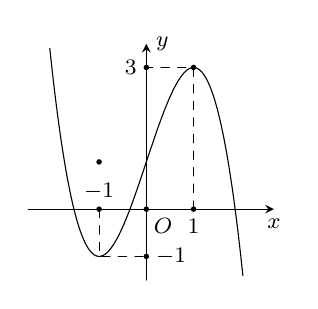
\begin{tikzpicture}[scale=1, font=\footnotesize, line join=round, line cap=round,>=stealth,x=0.6cm,y=0.6cm]
\def \xmin{-2.5};
\def \xmax{2.7};
\def \ymin{-1.5};
\def \ymax{3.5};
\draw[->] (\xmin, 0.) -- (\xmax,0.) node[anchor=north] {$x$};
\draw[->] (0.,\ymin) -- (0.,\ymax) node[anchor=west] {$y$};
\clip(\xmin+0.1,\ymin+0.1) rectangle (\xmax-0.1,\ymax-0.1);
\draw[smooth,samples=100,domain=\xmin:\xmax] plot(\x,{-(\x)^3+3*(\x)+1});
\draw[dashed] (-1,0) node[above]{$-1$} |- (0,-1)node[right]{$-1$} (1,0) node[below]{$1$} |- (0,3)node[left]{$3$};
\foreach \x/\y  in {-1/0,1/0,1/3,0/3,0/-1,-1/1}{\fill[black] (\x,\y) circle(1pt);}
\foreach \x/\y/\l/\g  in {0/0/O/-45}{\fill[black] (\x,\y) circle(1pt)+(\g:0.5) node{$\l$};}
\end{tikzpicture}}
\loigiai{
Từ đồ thị ta có giá trị cực đại của hàm số là $y_\text{CĐ}=3$.
}
\end{ex}

\begin{ex}%[Cau27-GV14]%[2D1Y2-2]
\immini{Cho hàm số có đồ thị như hình vẽ bên. Số điểm cực trị của hàm số đã cho là
\choice
{$1$}
{$2$}
{\True $3$}
{$0$}}{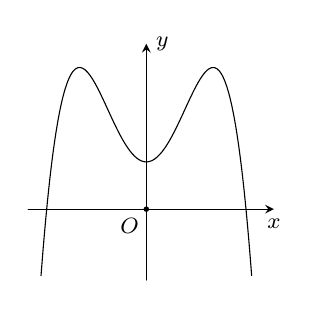
\begin{tikzpicture}[scale=1, font=\footnotesize, line join=round, line cap=round,>=stealth,x=0.6cm,y=0.6cm]
\def \xmin{-2.5};
\def \xmax{2.7};
\def \ymin{-1.5};
\def \ymax{3.5};
\draw[->] (\xmin, 0.) -- (\xmax,0.) node[anchor=north] {$x$};
\draw[->] (0.,\ymin) -- (0.,\ymax) node[anchor=west] {$y$};
\clip(\xmin+0.1,\ymin+0.1) rectangle (\xmax-0.1,\ymax-0.1);
\draw[smooth,samples=100,domain=\xmin:\xmax] plot(\x,{-0.5*(\x)^4+2*(\x)^2+1});

\foreach \x/\y/\l/\g  in {0/0/O/225}{\fill[black] (\x,\y) circle(1pt)+(\g:0.5) node{$\l$};}
\end{tikzpicture}}
\loigiai{
Từ đồ thị ta thấy hàm số $f(x)$ có $3$ điểm cực trị.
}
\end{ex}

\begin{ex}%[2D1Y2-2]
\immini{Cho hàm số $y=f(x)$ có đồ thị như hình vẽ sau. Khẳng định nào sau đây đúng?
\choice
{Hàm số có hai điểm cực trị âm và một điểm cực trị dương}
{\True Hàm số có hai điểm cực trị dương và một điểm cực trị âm}
{Hàm số đạt cực tiểu tại $x=-2$}
{Hàm số đat cưc đại tại $x=0$}}{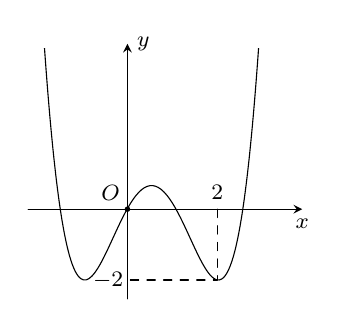
\begin{tikzpicture}[scale=1, font=\footnotesize, line join=round, line cap=round,>=stealth,x=0.6cm,y=0.6cm]
\def \xmin{-2.1};
\def \xmax{3.7};
\def \ymin{-1.9};
\def \ymax{3.5};
\draw[->] (\xmin, 0.) -- (\xmax,0.) node[anchor=north] {$x$};
\draw[->] (0.,\ymin) -- (0.,\ymax) node[anchor=west] {$y$};
\clip(\xmin+0.1,\ymin+0.1) rectangle (\xmax-0.1,\ymax-0.1);
\draw[smooth,samples=100,domain=\xmin:\xmax] plot(\x,{0.5*(\x-0.51)^4-2*(\x-0.51)^2+0.5});
\draw[dashed] (1.9,0) node[above]{$2$} |- (0,-1.5)node[left,xshift=2pt]{$-2$};
\foreach \x/\y/\l/\g  in {0/0/O/135}{\fill[black] (\x,\y) circle(1pt)+(\g:0.5) node{$\l$};}
\end{tikzpicture}}
\loigiai{
Từ đồ thị ta thấy hàm số  $y=f(x)$ có hai điểm cực trị dương và một điểm cực trị âm.
}
\end{ex}

\begin{ex}%[Cau27-GV14]%[2D1Y2-2]
\immini{Cho hàm số bậc bốn $y=f(x)$ có đồ thị hàm số như hình bên. Số điểm cực tiểu của hàm số đã cho là
\choice
{\True $2$}
{$1$}
{$3$}
{$0$}}{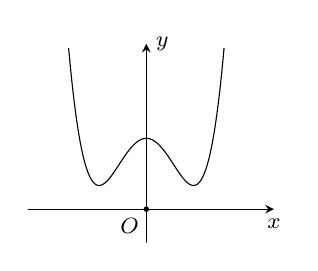
\begin{tikzpicture}[scale=1, font=\footnotesize, line join=round, line cap=round,>=stealth,x=0.6cm,y=0.6cm]
\def \xmin{-2.5};
\def \xmax{2.7};
\def \ymin{-0.7};
\def \ymax{3.5};
\draw[->] (\xmin, 0.) -- (\xmax,0.) node[anchor=north] {$x$};
\draw[->] (0.,\ymin) -- (0.,\ymax) node[anchor=west] {$y$};
\clip(\xmin+0.1,\ymin+0.1) rectangle (\xmax-0.1,\ymax-0.1);
\draw[smooth,samples=100,domain=\xmin:\xmax] plot(\x,{(\x)^4-2*(\x)^2+1.5});
\foreach \x/\y/\l/\g  in {0/0/O/225}{\fill[black] (\x,\y) circle(1pt)+(\g:0.5) node{$\l$};}
\end{tikzpicture}}
\loigiai{
Từ đồ thị ta thấy hàm số $y=f(x)$ có $2$ điểm cực tiểu.
}
\end{ex}

\begin{ex}%[Cau27-GV14]%[2D1Y2-2]
\immini{Cho hàm số $y=ax^3+bx^2+cx+d$ $(a,b,c,d \in \mathbb{R})$, có đồ thị như hình vẽ bên. Số điểm cực trị của hàm số đã cho là
\choice
{\True $2$}
{$0$}
{$3$}
{$1$}}{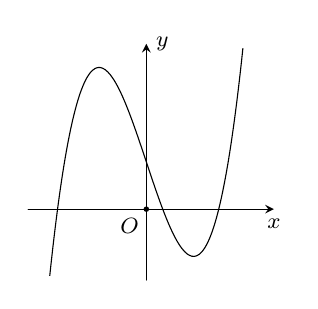
\begin{tikzpicture}[scale=1, font=\footnotesize, line join=round, line cap=round,>=stealth,x=0.6cm,y=0.6cm]
\def \xmin{-2.5};
\def \xmax{2.7};
\def \ymin{-1.5};
\def \ymax{3.5};
\draw[->] (\xmin, 0.) -- (\xmax,0.) node[anchor=north] {$x$};
\draw[->] (0.,\ymin) -- (0.,\ymax) node[anchor=west] {$y$};
\clip(\xmin+0.1,\ymin+0.1) rectangle (\xmax-0.1,\ymax-0.1);
\draw[smooth,samples=100,domain=\xmin:\xmax] plot(\x,{(\x)^3-3*(\x)+1});
\foreach \x/\y/\l/\g  in {0/0/O/225}{\fill[black] (\x,\y) circle(1pt)+(\g:0.5) node{$\l$};}
\end{tikzpicture}}
\loigiai{
Từ đồ thị ta thấy hàm số đã cho có $2$ điểm cực trị.
}
\end{ex}

\begin{ex}%[Cau27-GV14]%[2D1Y2-2]
\immini{Cho hàm số $y=f(x)$ có đồ thị như hình vẽ dưới đây. Giá trị cực tiểu của hàm số là
\choice
{$2$}
{$0$}
{$5$}
{\True $1$}}{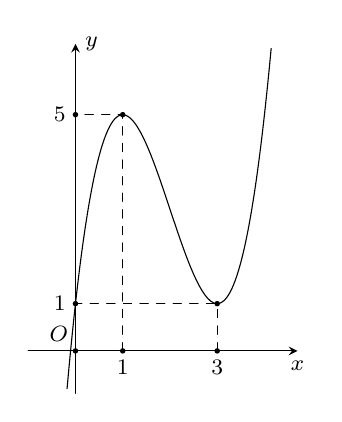
\begin{tikzpicture}[scale=1, font=\footnotesize, line join=round, line cap=round,>=stealth,x=0.6cm,y=0.6cm]
\def \xmin{-1.0};
\def \xmax{4.7};
\def \ymin{-0.9};
\def \ymax{6.5};
\draw[->] (\xmin, 0.) -- (\xmax,0.) node[anchor=north] {$x$};
\draw[->] (0.,\ymin) -- (0.,\ymax) node[anchor=west] {$y$};
\clip(\xmin+0.1,\ymin+0.1) rectangle (\xmax-0.1,\ymax-0.1);
\draw[smooth,samples=100,domain=\xmin:\xmax] plot(\x,{(\x-2)^3-3*(\x-2)+3});
\draw[dashed] (1,0) node[below]{$1$} |- (0,5)node[left]{$5$} (3,0) node[below]{$3$} |- (0,1)node[left]{$1$};
\foreach \x/\y  in {1/5,3/1,1/0,3/0,0/1,0/5}{\fill[black] (\x,\y) circle(1pt);}
\foreach \x/\y/\l/\g  in {0/0/O/135}{\fill[black] (\x,\y) circle(1pt)+(\g:0.5) node{$\l$};}
\end{tikzpicture}}
\loigiai{
Từ đồ thị ta thấy giá trị cực tiểu của hàm số là $y_\text{CT}=1$.
}
\end{ex}

\begin{ex}%[Cau27-GV14]%[2D1Y2-2]
\immini{Cho hàm số $y=f(x)$ xác định, liên tục trên đoạn $[-4;0]$ và có đồ thị là đường cong trong hình vẽ bên. Hàm số $f(x)$ đạt cực tiểu tại điểm nào dưới đây?
\choice
{$x=-2$}
{\True $x=-1$}
{$x=-3$}
{$x=2$}}{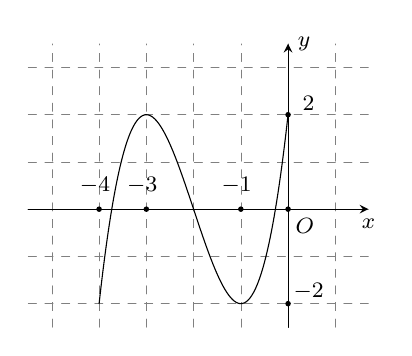
\begin{tikzpicture}[scale=1, font=\footnotesize, line join=round, line cap=round,>=stealth,x=0.6cm,y=0.6cm]
\def \xmin{-5.5};
\def \xmax{1.7};
\def \ymin{-2.5};
\def \ymax{3.5};
\draw[step=0.6cm,gray,very thin,dashed] (\xmin,\ymin) grid (\xmax,\ymax);
\draw[->] (\xmin, 0.) -- (\xmax,0.) node[anchor=north] {$x$};
\draw[->] (0.,\ymin) -- (0.,\ymax) node[anchor=west] {$y$};
\clip(\xmin+0.1,\ymin+0.1) rectangle (\xmax-0.1,\ymax-0.1);
\draw[smooth,samples=100,domain=-4:0] plot(\x,{(\x+2)^3-3*(\x+2)});
\foreach \x/\y/\l/\g  in {0/0/O/-45,-1/0/-1/100,-3/0/-3/100,0/2/2/30,0/-2/-2/30,-4/0/-4/100}{\fill[black] (\x,\y) circle(1pt)+(\g:0.5) node{$\l$};}
\end{tikzpicture}}
\loigiai
{Từ đồ thị ta thấy hàm số đã cho đạt cực tiểu tại $x=-1$.
}
\end{ex}

\begin{ex}%[Cau27-GV14]%[2D1Y2-2]
\immini{Cho hàm số $y=f(x)$ liên tục trên đoạn $[0;4]$ có đồ thị như hình vẽ bên. Mệnh đề nào sau đây đúng?
\choice
{\True Hàm số đạt cực tiểu tại $x=3$}
{Hàm số đạt cực tiểu tại $x=0$}
{Hàm số đạt cực đại tại $x=4$}
{Hàm số đạt cực đại tại $x=2$}}{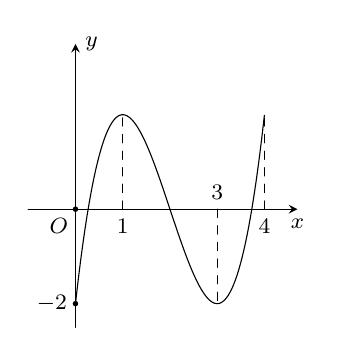
\begin{tikzpicture}[scale=1, font=\footnotesize, line join=round, line cap=round,>=stealth,x=0.6cm,y=0.6cm]
\def \xmin{-1.0};
\def \xmax{4.7};
\def \ymin{-2.5};
\def \ymax{3.5};
\draw[->] (\xmin, 0.) -- (\xmax,0.) node[anchor=north] {$x$};
\draw[->] (0.,\ymin) -- (0.,\ymax) node[anchor=west] {$y$};
\clip(\xmin+0.1,\ymin+0.1) rectangle (\xmax-0.1,\ymax-0.1);
\draw[smooth,samples=100,domain=0:4] plot(\x,{(\x-2)^3-3*(\x-2)});
\draw[dashed] (1,0) node[below]{$1$} -- (1,2) (3,0) node[above]{3} -- (3,-2) (4,0) node[below]{$4$} -- (4,2);
\foreach \x/\y/\l/\g  in {0/0/O/225,0/-2/-2/-180}{\fill[black] (\x,\y) circle(1pt)+(\g:0.5) node{$\l$};}
\end{tikzpicture}}
\loigiai
{Mệnh đề ``Hàm số đạt cực tiểu tại $x=3$'' là mệnh đề đúng.
}
\end{ex}

\begin{ex}%[Cau27-GV14]%[2D1Y2-2]
\immini{ Cho hàm số  $f(x)$ có đồ thị như hình vẽ bên. Số điểm cực đại của hàm số đã cho là
\choice
{$0$}
{\True $1$}
{$2$}
{$3$}}{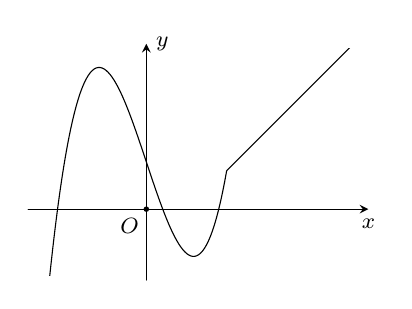
\begin{tikzpicture}[scale=1, font=\footnotesize, line join=round, line cap=round,>=stealth,x=0.6cm,y=0.6cm]
\def \xmin{-2.5};
\def \xmax{4.7};
\def \ymin{-1.5};
\def \ymax{3.5};
\draw[->] (\xmin, 0.) -- (\xmax,0.) node[anchor=north] {$x$};
\draw[->] (0.,\ymin) -- (0.,\ymax) node[anchor=west] {$y$};
\clip(\xmin+0.1,\ymin+0.1) rectangle (\xmax-0.1,\ymax-0.1);
\draw[smooth,samples=100,domain=\xmin:1.7] plot(\x,{(\x)^3-3*(\x)+1});
\draw[smooth,samples=100,domain=1.7:\xmax] plot(\x,{(\x)-0.887});

\foreach \x/\y/\l/\g  in {0/0/O/225}{\fill[black] (\x,\y) circle(1pt)+(\g:0.5) node{$\l$};}
\end{tikzpicture}}
\loigiai
{Từ đồ thị ta thấy hàm số đã cho có $1$ điểm cực đại.
}
\end{ex}
\Closesolutionfile{ans}
%======================
\subsection{Bảng đáp án}
\inputansbox{8}{ans/ANS-DANG-27}
